\documentclass{ximera}

%% You can put user macros here
%% However, you cannot make new environments

\listfiles

\graphicspath{{./}{firstExample/}{secondExample/}}

\usepackage{tikz}
\usepackage{tkz-euclide}
\usepackage{tikz-3dplot}
\usepackage{tikz-cd}
\usetikzlibrary{shapes.geometric}
\usetikzlibrary{arrows}
\usetikzlibrary{decorations.pathmorphing,patterns}
\usetkzobj{all}
\pgfplotsset{compat=1.13} % prevents compile error.

\renewcommand{\vec}[1]{\mathbf{#1}}
\newcommand{\RR}{\mathbb{R}}
\newcommand{\dfn}{\textit}
\newcommand{\dotp}{\cdot}
\newcommand{\id}{\text{id}}
\newcommand\norm[1]{\left\lVert#1\right\rVert}
 
\newtheorem{general}{Generalization}
\newtheorem{initprob}{Exploration Problem}

\tikzstyle geometryDiagrams=[ultra thick,color=blue!50!black]

\usepackage{mathtools}




\title{6.3 The $RLC$ Circuit}


\begin{document}

\begin{abstract}
We study electric circuits as an application of second order linear differential equations.
\end{abstract}

\maketitle

\section*{The $RLC$ Circuit}

In this section we consider the \textit{RLC circuit}, shown
schematically in the figure below. 

\begin{image}
  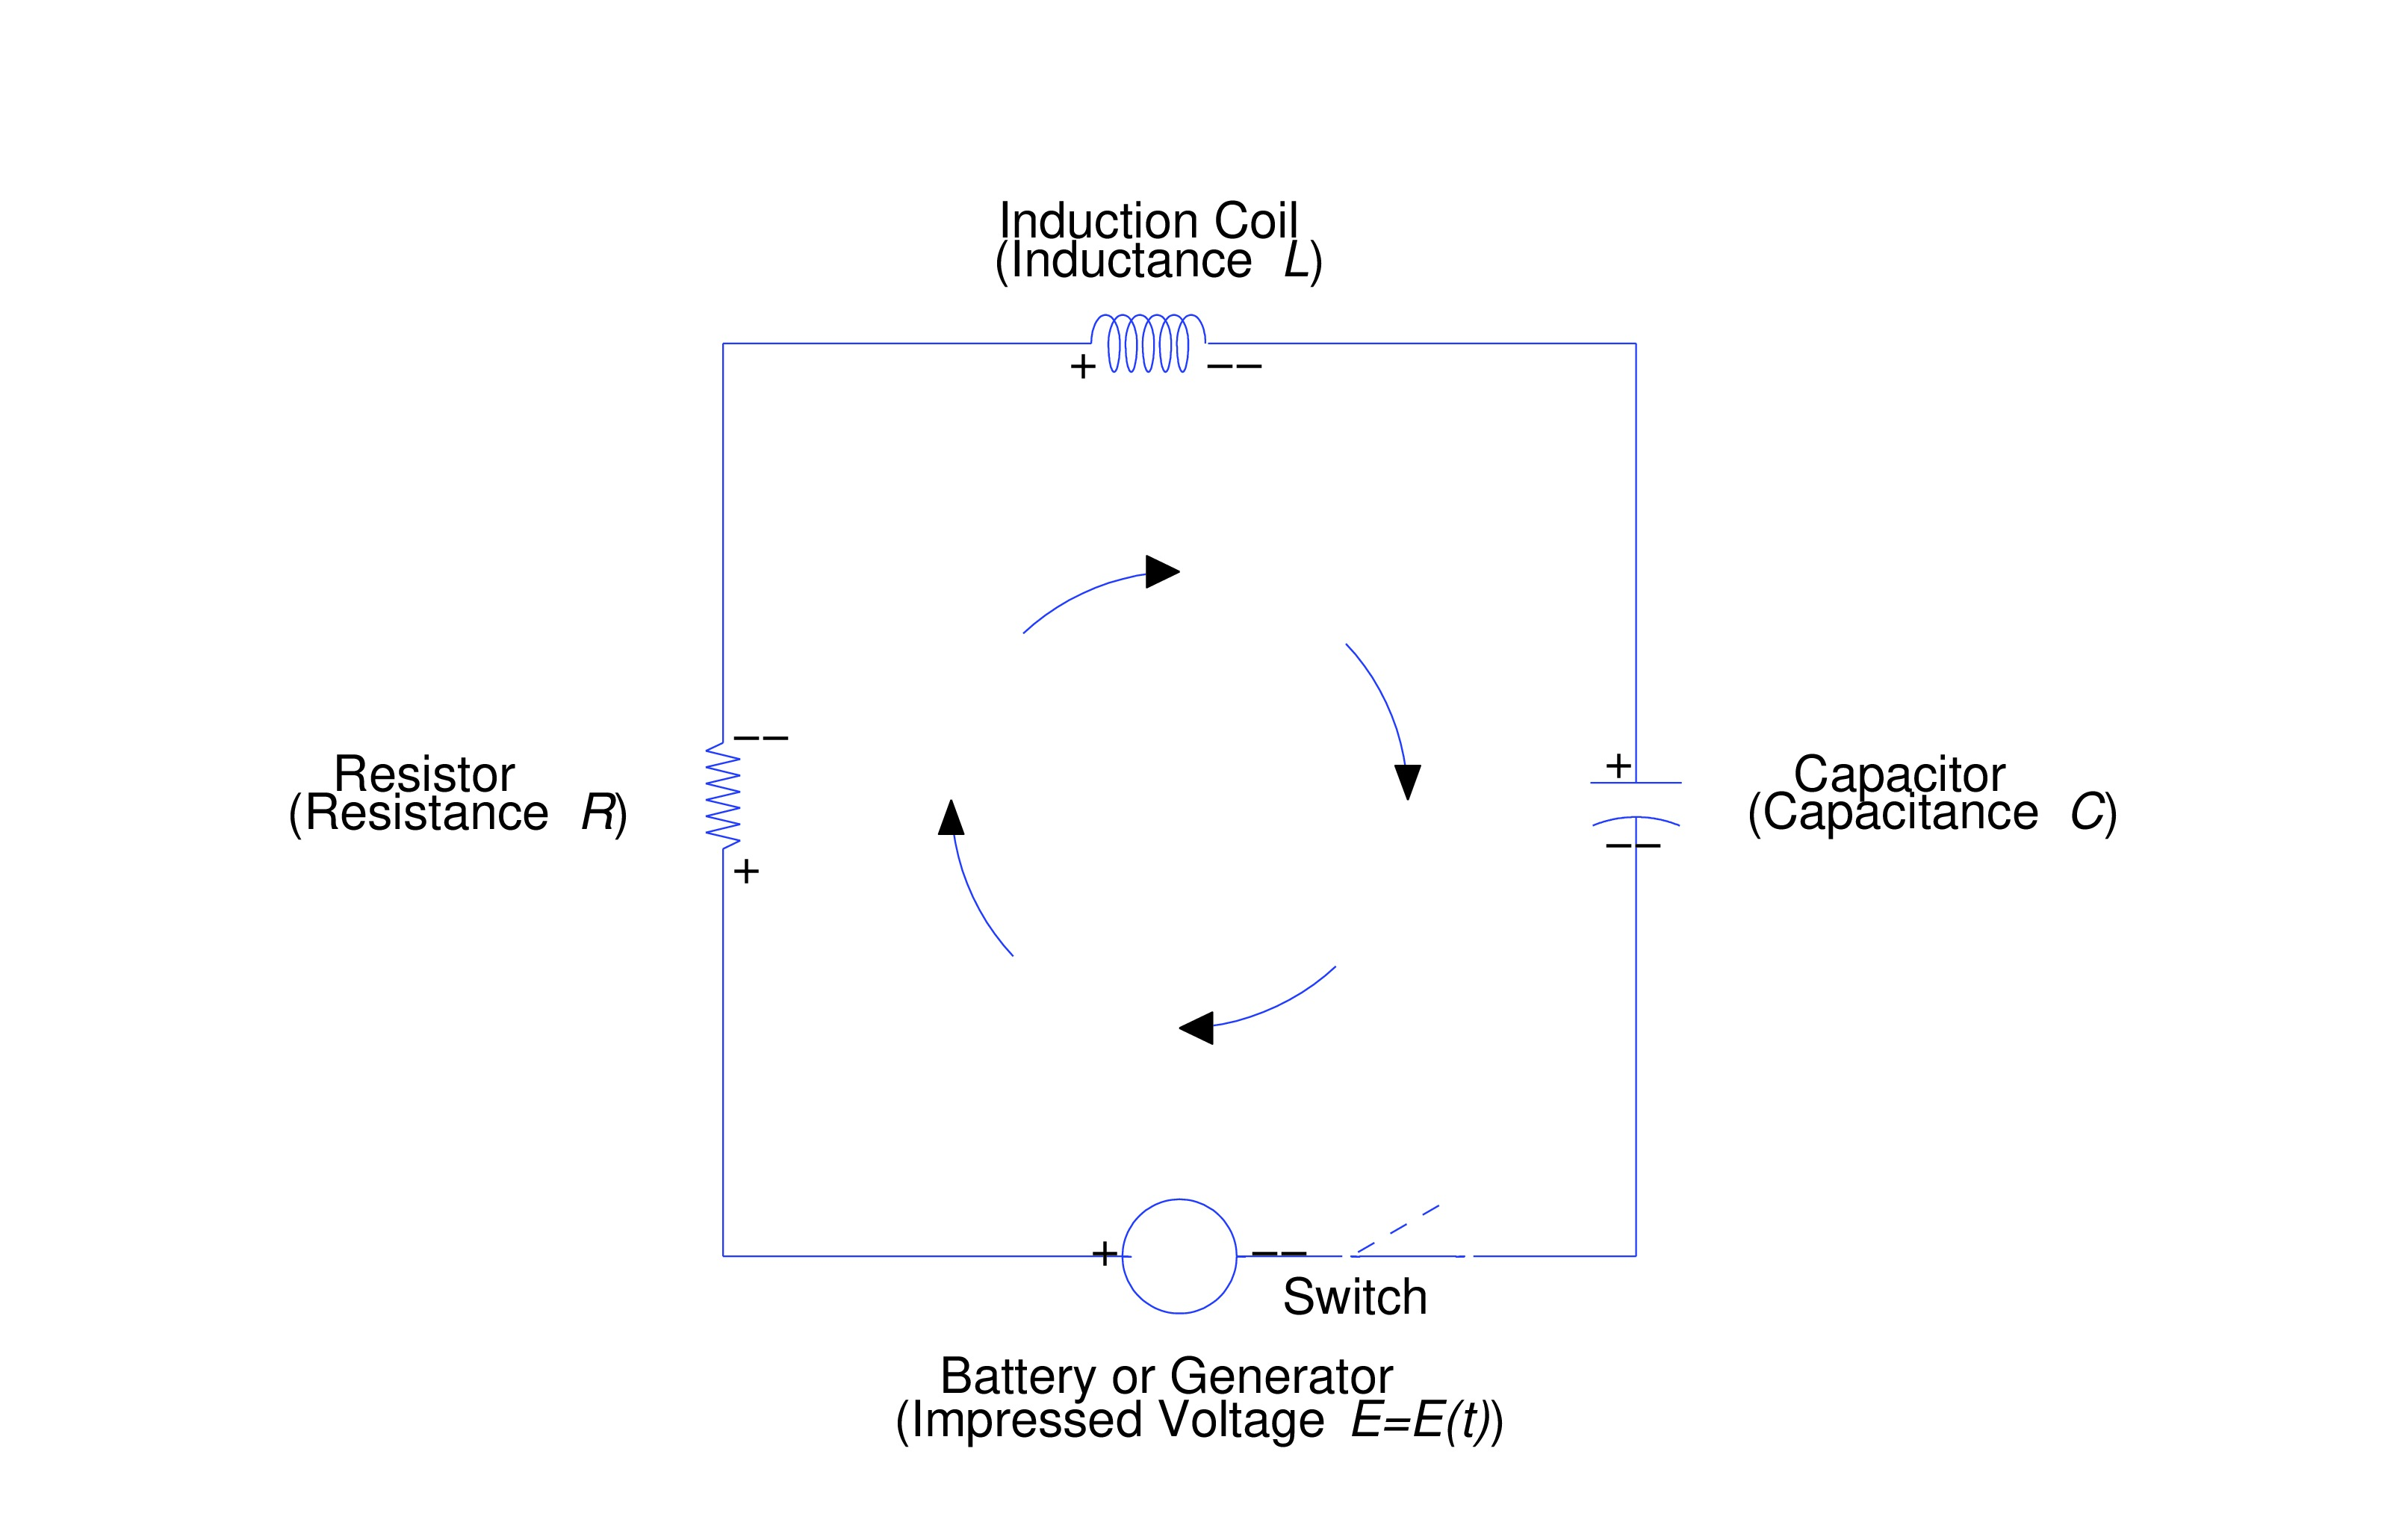
\includegraphics[height=1.5in]{fig060301.jpg} 
\end{image}

As we'll see, the $RLC$
circuit is an electrical analog of a spring-mass system with
damping.

Nothing happens while the switch is open (dashed line). When the
switch is closed (solid line) we say that the \textit{circuit is closed}. Differences in electrical potential in a closed circuit
cause current to flow in the circuit. The battery or generator, shown in the figure,
 creates a difference in electrical potential
$E=E(t)$ between its two terminals, which we've marked arbitrarily as
positive and negative. (We could just as well interchange the
markings.) We'll say that $E(t)>0$ if the potential at the positive
terminal is greater than the potential at the negative terminal,
$E(t)<0$ if the potential at the positive terminal is less than the
potential at the negative terminal, and $E(t)=0$ if the potential is
the same at the two terminals. We call $E$ the \textit{impressed
voltage}.

At any  time $t$, the same current flows in all points of the
circuit. We denote current by $I=I(t)$. We say that $I(t)>0$ if the
direction of flow is around the circuit from the positive terminal of
the battery or generator back to the negative terminal, as indicated
by the arrows in the figure,   $I(t)<0$ if the flow is in the
opposite direction, and $I(t)=0$ if no current flows at time $t$.

Differences in potential occur at the resistor, induction coil, and
capacitor. Note that the two sides of each
of these components are also identified as positive and negative. The
\textit{voltage drop across}  each component is defined to be the
potential on the positive side of the component minus the potential on
the negative side. This terminology is somewhat misleading, since
``drop'' suggests a decrease even though changes in potential are
signed quantities and therefore may be increases. Nevertheless,
we'll go along with tradition and call them voltage drops.
The voltage drop across the resistor, as shown in the figure, is given
by
\begin{equation} \label{eq:6.3.1}
V_R=IR,
\end{equation}
where $I$ is current and $R$ is a positive constant, the \textit{resistance} of the resistor. The voltage drop across the induction
coil is given by
\begin{equation} \label{eq:6.3.2}
V_I=L\frac{dI}{dt}=LI',
\end{equation}
where $L$ is a positive constant, the \textit{inductance} of the coil.

A capacitor stores electrical charge $Q=Q(t)$, which is related to
the current in the circuit by the equation
\begin{equation} \label{eq:6.3.3}
Q(t)=Q_0+\int_0^tI(\tau)\,d\tau,
\end{equation}
where $Q_0$ is the charge on the capacitor at $t=0$. The voltage drop
across a capacitor is given by
\begin{equation} \label{eq:6.3.4}
V_C=\frac{Q}{C},
\end{equation}
where $C$ is a positive constant, the \textit{capacitance} of the
capacitor.

The following table names the units for the quantities that we've
discussed. The units are defined so that
\begin{eqnarray*}
1\,\mbox{volt}&=&1\,\mbox{ampere}\cdot1\,\mbox{ohm}\\
&=&1\,\mbox{henry}\cdot1\,\mbox{ampere}/\mbox{second}\\
&=&1\,\mbox{coulomb}/\mbox{farad}
\end{eqnarray*}
and
\begin{eqnarray*}
1\,\mbox{ampere}&=&1\,\mbox{coulomb}/\mbox{second}.
\end{eqnarray*}

\begin{center}
\begin{tabular}{|c|c|c|}
\hline
 {\bf Symbol}&{\bf Name}& {\bf Unit}\\\hline
$E$  &  Impressed Voltage & volt  \\\hline
$I$ & Current & ampere \\\hline
$Q$ & Charge & coulomb\\\hline
$R$ & Resistance& ohm\\\hline
$L$ & Inductance& henry\\\hline
$C$ & Capacitance&farad\\\hline
\end{tabular}
\end{center}

According to
\href{http://www-history.mcs.st-and.ac.uk/Mathematicians/Kirchhoff.html}
{Kirchoff's Law}, the sum of
the voltage drops in a closed $RLC$ circuit equals the impressed
voltage. Therefore, from (\ref{eq:6.3.1}), (\ref{eq:6.3.2}), and (\ref{eq:6.3.4}),
\begin{equation} \label{eq:6.3.5}
 LI'+RI+\frac{1}{C}Q=E(t).
\end{equation}
This equation contains two unknowns, the current $I$ in the
circuit and the charge $Q$ on the capacitor. However, (\ref{eq:6.3.3})
implies that $Q'=I$, so (\ref{eq:6.3.5}) can be converted into the second
order equation
\begin{equation} \label{eq:6.3.6}
 LQ''+RQ'+\frac{1}{C}Q=E(t)
\end{equation}
in $Q$. To find the current flowing in an $RLC$ circuit, we solve
(\ref{eq:6.3.6}) for $Q$ and then differentiate the solution to obtain
$I$.

In Trench \href{https://ximera.osu.edu/ode/main/springProblemsI/springProblemsI}{6.1} and \href{https://ximera.osu.edu/ode/main/springProblemsII/springProblemsII}{6.2} we encountered the
equation
\begin{equation} \label{eq:6.3.7}
my''+cy'+ky=F(t)
\end{equation}
in connection with spring-mass systems. Except for notation this
equation is the same as (\ref{eq:6.3.6}). The correspondence between
electrical and mechanical quantities connected with (\ref{eq:6.3.6}) and
(\ref{eq:6.3.7}) is shown in the table below.

\begin{center}
\begin{tabular}{|lc|lc|}\hline
\multicolumn{2}{|c|}{\bf Electrical}&
\multicolumn{2}{c|}{\bf Mechanical}\\\hline
charge& $Q$& displacement&$y$\\\hline
curent&$I$&velocity&$y'$\\\hline
impressed voltage&$E(t)$&external force&$F(t)$\\\hline
inductance&$L$&Mass&$m$\\\hline
resistance&$R$&damping&$c$\\\hline
1/capacitance&$1/C$&spring constant&$k$\\\hline
\end{tabular}
\end{center}

The equivalence between (\ref{eq:6.3.6}) and (\ref{eq:6.3.7}) is an example of
how mathematics unifies fundamental similarities in diverse physical
phenomena. Since we've already studied the properties of solutions of
(\ref{eq:6.3.7}) in In Trench \href{https://ximera.osu.edu/ode/main/springProblemsI/springProblemsI}{6.1} and \href{https://ximera.osu.edu/ode/main/springProblemsII/springProblemsII}{6.2}, we
can obtain
results concerning solutions of (\ref{eq:6.3.6}) by simply changing
notation, according to the table.

\subsection*{Free Oscillations}

We say that an $RLC$ circuit is in \textit{free oscillation} if $E(t)=0$
for $t>0$, so that (\ref{eq:6.3.6}) becomes
\begin{equation} \label{eq:6.3.8}
LQ''+RQ'+\frac{1}{C}Q=0.
\end{equation}
The characteristic equation of (\ref{eq:6.3.8}) is
$$
Lr^2+Rr+\frac{1}{C}=0,
$$
with roots
\begin{equation}\label{eq:6.3.9}
r_1=\frac{-R-\sqrt{R^2-4L/C}}{2L}\quad\mbox{and}\quad r_2=
\frac{-R+\sqrt{R^2-4L/C}}{2L}.
\end{equation}
There are three cases to consider, all analogous to the cases
considered in In \href{https://ximera.osu.edu/ode/main/springProblemsII/springProblemsII}{Trench 6.2} for free vibrations of a damped
spring-mass system.

Case 1.
The oscillation is \textit{underdamped} if $R<\sqrt{4L/C}$. In this
case, $r_1$ and $r_2$ in (\ref{eq:6.3.9}) are complex conjugates, which we
write as
$$
r_1=-\frac{R}{2L}+i\omega_1\quad\mbox{and}\quad r_2=-\frac{R}{2L}-i\omega_1,
$$
where
$$
\omega_1=\frac{\sqrt{4L/C-R^2}}{2L}.
$$
The general solution of  (\ref{eq:6.3.8})  is
$$
Q=e^{-Rt/2L}(c_1\cos\omega_1 t+c_2\sin\omega_1 t),
$$
which we can write as
\begin{equation}\label{eq:6.3.10}
Q=Ae^{-Rt/2L}\cos(\omega_1 t-\phi),
\end{equation}
 where
$$
A=\sqrt{c_1^2+c_2^2},\quad A\cos\phi=c_1,\quad\mbox{and}\quad A\sin\phi=c_2.
$$
In the idealized case where $R=0$, the solution (\ref{eq:6.3.10})
reduces to
$$
Q=A\cos\left(\frac{t}{\sqrt{LC}}-\phi\right),
$$
which is analogous to  the simple harmonic motion of an undamped
spring-mass system in free vibration.

Actual $RLC$ circuits are usually underdamped, so the case we've just
considered is the most important. However, for completeness we'll
consider the other two possibilities.

Case 2.
The oscillation is \textit{overdamped} if $R>\sqrt{4L/C}$. In this case,
the zeros $r_1$ and $r_2$ of the characteristic polynomial are real,
with $r_1<r_2<0$ (see (\ref{eq:6.3.9})), and the general solution of
(\ref{eq:6.3.8}) is
\begin{equation}\label{eq:6.3.11}
Q=c_1e^{r_1t}+c_2e^{r_2t}.
\end{equation}

Case 3.
The oscillation is \textit{critically damped} if $R=\sqrt{4L/C}$. In
this case, $r_1=r_2=-R/2L$ and the general solution of (\ref{eq:6.3.8}) is
\begin{equation}\label{eq:6.3.12}
Q=e^{-Rt/2L}(c_1+c_2t).
\end{equation}

If $R\neq 0$, the exponentials in (\ref{eq:6.3.10}), (\ref{eq:6.3.11}),
and
(\ref{eq:6.3.12}) are negative, so the solution of any homogeneous initial
value problem
$$
 LQ''+RQ'+\frac{1}{C}Q=0,\quad Q(0)=Q_0,\quad Q'(0)=I_0,
$$
approaches zero exponentially as $t\rightarrow\infty$. Thus, all such
solutions are \textit{transient}, in the sense defined
In \href{https://ximera.osu.edu/ode/main/springProblemsII/springProblemsII}{Trench 6.2} in the discussion of forced vibrations of a
spring-mass system with damping.

\begin{example}\label{example:6.3.1}
At $t=0$ a current of 2 amperes flows in an $RLC$ circuit with
resistance $R=40$ ohms, inductance $L=.2$ henrys, and capacitance
$C=10^{-5}$ farads. Find the current flowing in the circuit at $t>0$
if the initial charge on the capacitor is 1 coulomb. Assume that
$E(t)=0$ for $t>0$.

\begin{explanation} The equation for the charge $Q$ is $$\frac{1}{5}Q''+40Q'+10000Q=0, $$ or
\begin{equation} \label{eq:6.3.13}
Q''+200Q'+50000Q=0.
\end{equation}
Therefore we must solve the initial value problem
\begin{equation} \label{eq:6.3.14}
Q''+200Q'+50000Q=0,\quad Q(0)=1,\quad Q'(0)=2.
\end{equation}
The desired current is the derivative of the solution of this initial
value problem.

The characteristic equation of (\ref{eq:6.3.13}) is
$$
r^2+200r+50000=0,
$$
which has complex zeros $r=-100\pm200i$. Therefore the general
solution of (\ref{eq:6.3.13}) is
\begin{equation} \label{eq:6.3.15}
Q=e^{-100t}(c_1\cos200t+c_2\sin200t).
\end{equation}
Differentiating this and collecting like terms yields
\begin{equation} \label{eq:6.3.16}
Q'=-e^{-100t}\left[(100c_1-200c_2)\cos200t+
(100c_2+200c_1)\sin200t\right].
\end{equation}
To find the solution of the initial value problem (\ref{eq:6.3.14}),
we set $t=0$ in (\ref{eq:6.3.15}) and (\ref{eq:6.3.16}) to obtain
$$
c_1=Q(0)=1\quad\mbox{and}\quad   -100c_1+200c_2=Q'(0)=2;
$$
therefore, $c_1=1$ and $c_2=51/100$, so
$$
Q=e^{-100t}\left(\cos200t+\frac{51}{100}\sin200t\right)
$$
is the solution of (\ref{eq:6.3.14}).
Differentiating this yields
$$
I=e^{-100t}(2\cos200t-251\sin200t).
$$
\end{explanation}
\end{example}

\subsection*{Forced Oscillations With Damping}

An initial value problem for (\ref{eq:6.3.6})  has the form
\begin{equation} \label{eq:6.3.17}
 LQ''+RQ'+\frac{1}{C}Q=E(t),\quad Q(0)=Q_0,\quad Q'(0)=I_0,
\end{equation}
where $Q_0$ is the initial charge on the capacitor and $I_0$ is the
initial current in the circuit. We've already seen that if $E\equiv0$
then all solutions of (\ref{eq:6.3.17}) are transient. If
$E\not\equiv0$, we know that the solution of (\ref{eq:6.3.17}) has
the form $Q=Q_c+Q_p$, where $Q_c$ satisfies the complementary
equation, and approaches zero exponentially as $t\rightarrow\infty$ for any
initial conditions , while $Q_p$ depends only on $E$ and is
independent of the initial conditions. As in the case of forced
oscillations of a spring-mass system with damping, we call $Q_p$ the \textit{steady state} charge on the capacitor of the $RLC$ circuit. Since
$I=Q'=Q_c'+Q_p'$ and $Q_c'$ also tends to zero exponentially as
$t\rightarrow\infty$, we say that $I_c=Q'_c$ is the \textit{transient} current
and $I_p=Q_p'$ is the \textit{steady state} current. In most
applications we're interested only in the steady state charge and
current.

\begin{example}\label{example:6.3.2}
Find the amplitude-phase form of the steady state current in the $RLC$
circuit in the figure if the impressed voltage, provided by
an alternating current generator, is $E(t)=E_0\cos\omega t$.

\begin{image}
  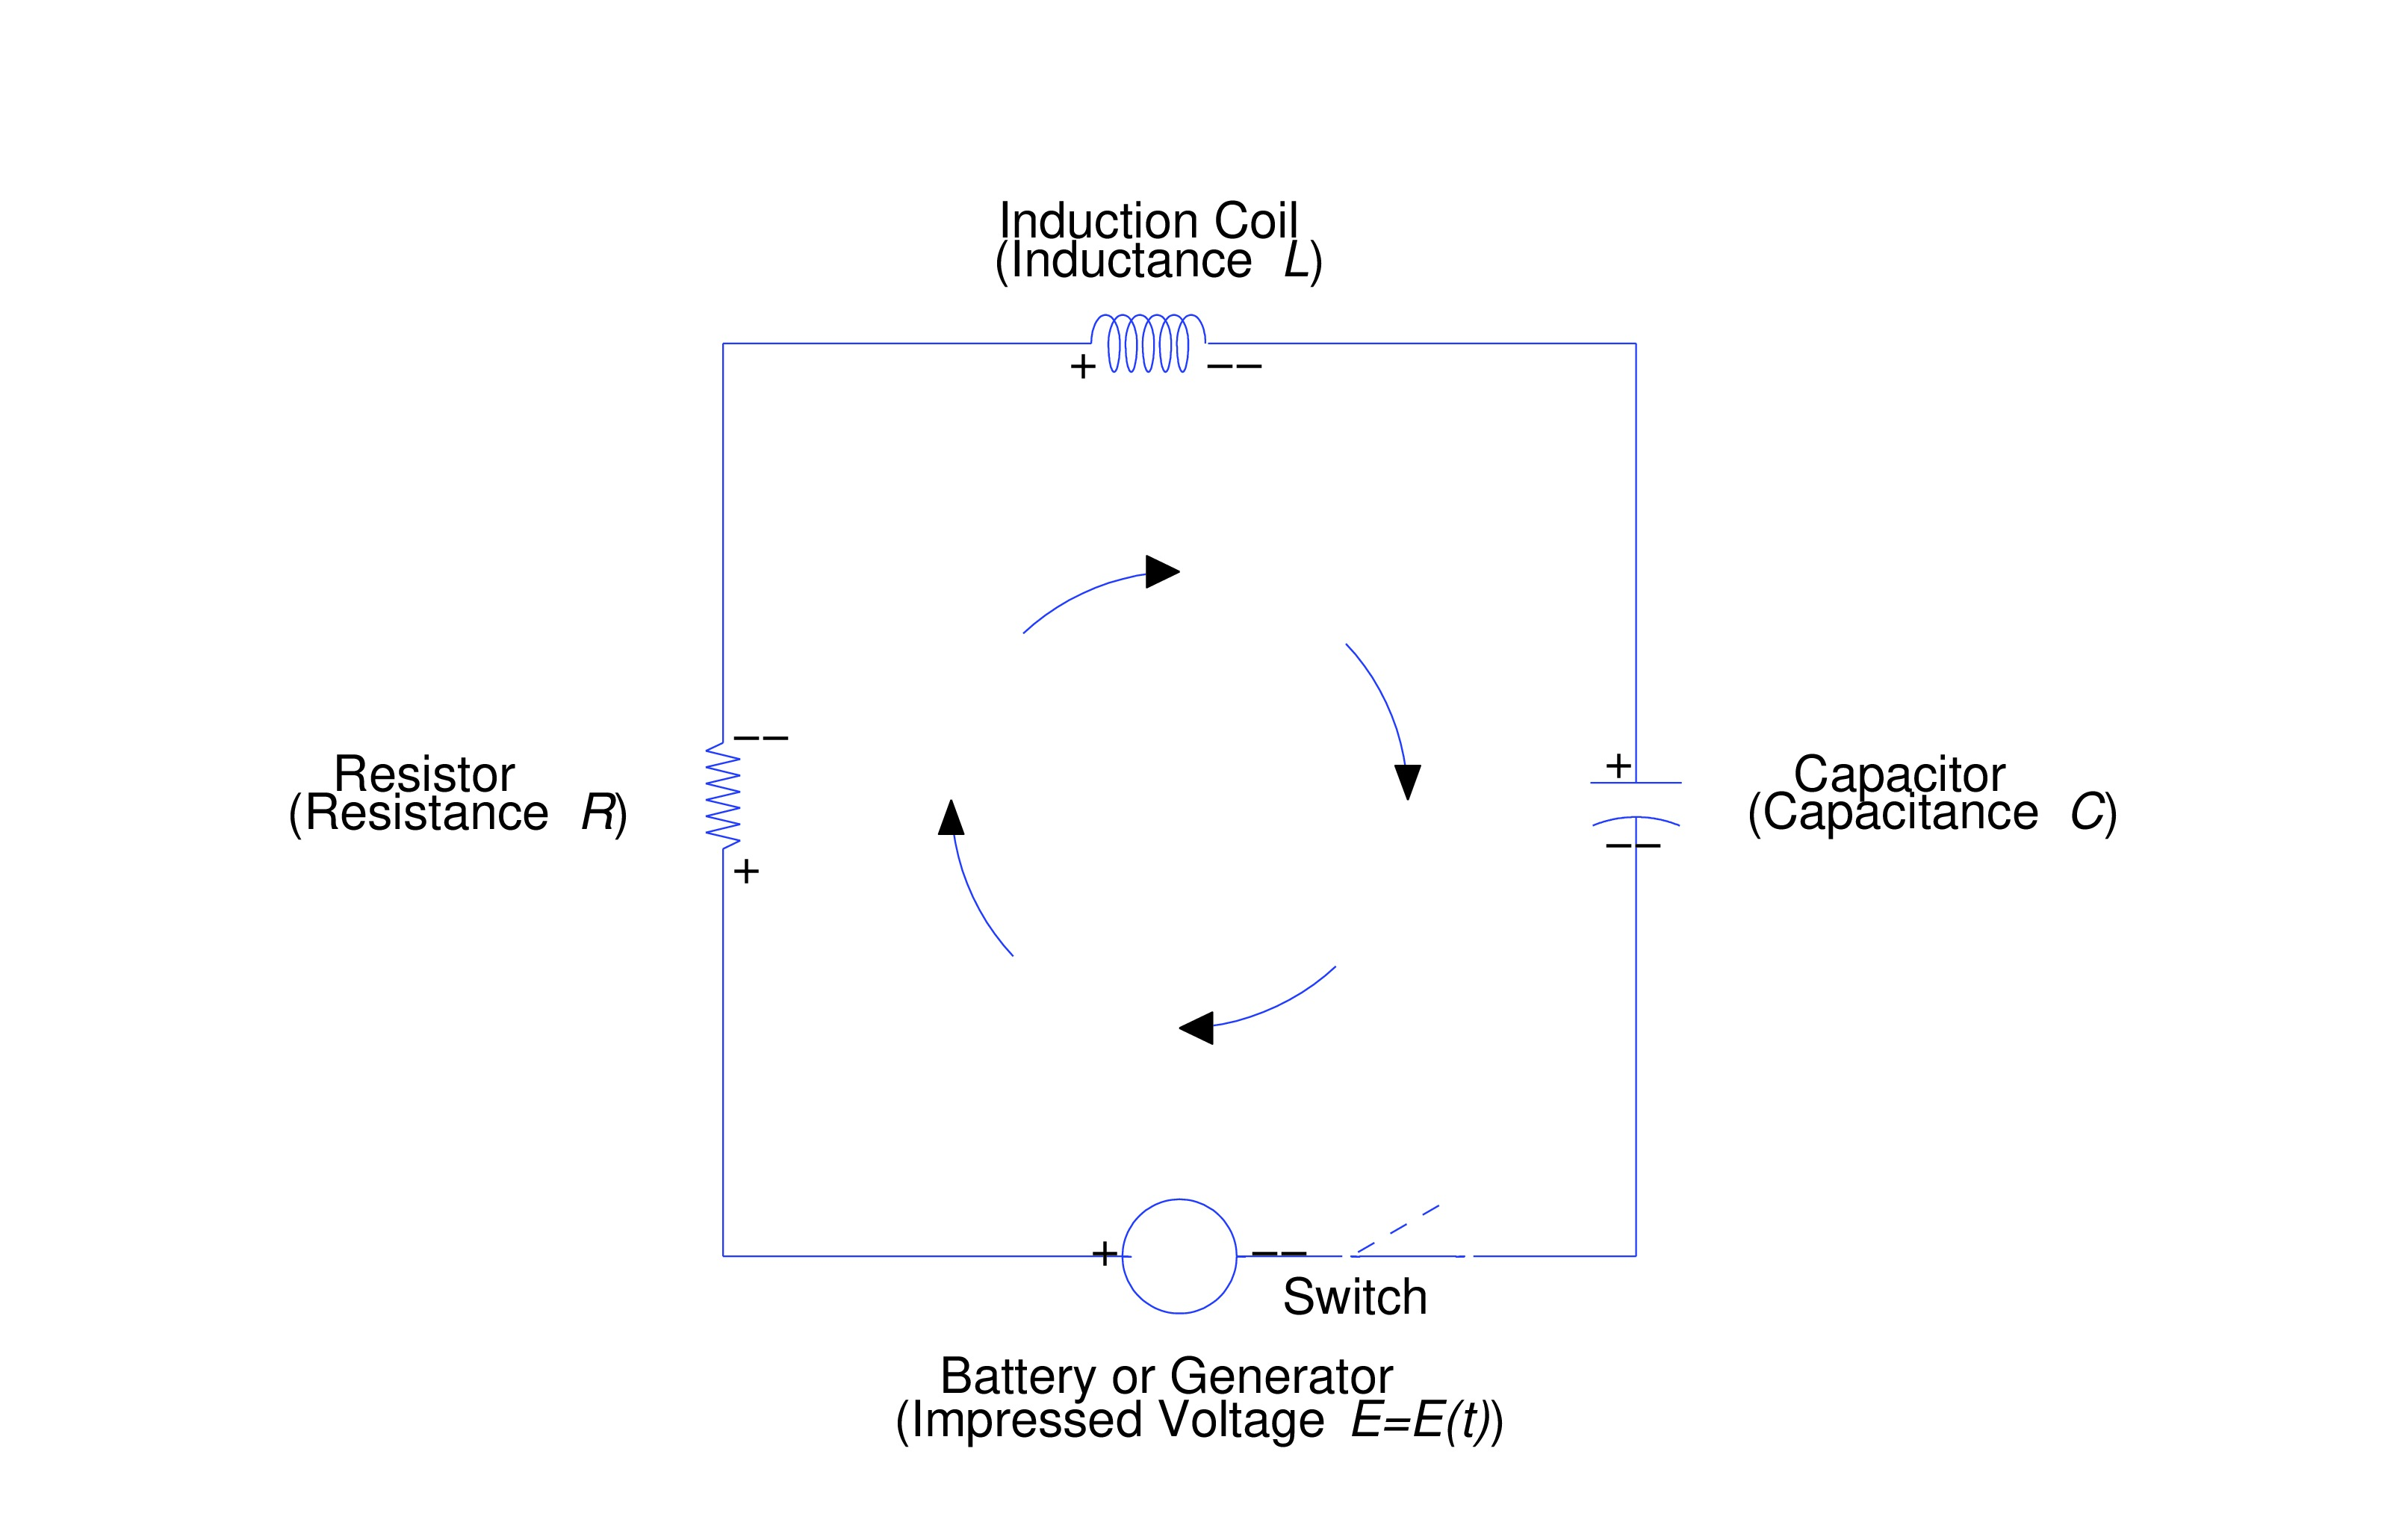
\includegraphics[height=1.5in]{fig060301.jpg} 
\end{image}

\begin{explanation}
We'll first find the steady state charge on the capacitor as
a particular solution of
$$
LQ''+RQ'+\frac{1}{C}Q=E_0\cos\omega t.
$$
To do, this we'll simply reinterpret a result obtained in
In \href{https://ximera.osu.edu/ode/main/springProblemsII/springProblemsII}{Trench 6.2}, where we found that the steady state solution of
$$
my''+cy'+ky=F_0\cos\omega t
$$
is
$$
y_p=\frac{F_0}{\sqrt{(k-m\omega^2)^2+c^2\omega^2}}
\cos(\omega t-\phi),
$$
where
$$
\cos\phi=\frac{k-m\omega^2}{\sqrt
{(k-m\omega^2)^2+c^2\omega^2}}\quad\mbox{and}\quad
\sin\phi=\frac{c\omega}{\sqrt{(k-m\omega^2)^2+c^2\omega^2}}.
$$
(See Equations~\eqref{eq:6.2.14} and \eqref{eq:6.2.15}.) By making the
appropriate changes in the symbols, according to the table,

\begin{center}
\begin{tabular}{|lc|lc|}\hline
\multicolumn{2}{|c|}{\bf Electrical}&
\multicolumn{2}{c|}{\bf Mechanical}\\\hline
charge& $Q$& displacement&$y$\\\hline
curent&$I$&velocity&$y'$\\\hline
impressed voltage&$E(t)$&external force&$F(t)$\\\hline
inductance&$L$&Mass&$m$\\\hline
resistance&$R$&damping&$c$\\\hline
1/capacitance&$1/C$&spring constant&$k$\\\hline
\end{tabular}
\end{center}

yields the steady state charge
$$
Q_p=\frac{E_0}{\sqrt{(1/C-L\omega^2)^2+R^2\omega^2}}\cos(\omega
t-\phi),
$$
where
$$
\cos\phi=\frac{1/C-L\omega^2}{\sqrt{(1/C-L\omega^2)^2+R^2\omega^2}}
\quad\mbox{and}\quad
\sin\phi=\frac{R\omega}{\sqrt{(1/C-L\omega^2)^2+R^2\omega^2}}.
$$
 Therefore the steady state current in the circuit
is
$$
I_p=Q_p'=
-\frac{\omega E_0}{\sqrt{(1/C-L\omega^2)^2+R^2\omega^2}}\sin(\omega
t-\phi).
$$
\end{explanation}
\end{example}
\section*{Text Source}
Trench, William F., "Elementary Differential Equations" (2013). Faculty Authored and Edited Books \& CDs. 8. (CC-BY-NC-SA)

\href{https://digitalcommons.trinity.edu/mono/8/}{https://digitalcommons.trinity.edu/mono/8/}

\end{document}


